
\section{Syntax and Semantics}\label{sec:form}
In this section we will describe our formalization of GraphQL in Coq. We will follow a similar structure as the previous section. We start by defining a schema and its properties, then the graph data model and finally we review queries and their semantics.

\td{The definitions consist of around 3700 loc and 1400 of lemmas}.

\subsection{GraphQL Schema}

The GraphQL schema is pretty straightforward to define from the Spec. It consists of a collection of type definitions and a root query operation type. The Spec uses a structure called \texttt{schema} where it defines the root operation types (query, mutation and subscription) and \textit{separately} the type definitions. We opted to define them all in a single structure.

\begin{minted}{coq}
Structure graphQLSchema := GraphQLSchema {
    query_type : Name;
    type_definitions : seq TypeDefinition
}.
\end{minted}

Similarly, for type definitions we follow the grammar as specified in the Spec. Figure \ref{fig:types_def} shows the grammar and the corresponding implementation in Coq. As can be seen in the figure, we tried to match the Spec's definition as much as possible. This eyeball correspondence gives us a degree of confidence about the implementation.  % We currently do not include the \textit{Input Object} types, as well as anything related to \textit{introspection}.

Although both definitions are straightforward, they allow building invalid schemas. For instance, it is possible to build an Object that implements scalar types, an Interface with no fields or use an nonexistent type as the query type. We therefore require a notion of \textit{well-formedness} of a schema.

\begin{definition}
A GraphQL schema is \textit{well-formed} if it satisfies the following conditions:
\begin{itemize}
    \item Its root query type is defined and is an Object type.
    \item There are no duplicated type names.
    \item Every type definition is \textit{well-formed}.
\end{itemize}
\end{definition}

We can then proceed to define a structure that encapsulates this notion, by passing both a schema and a proof of its \textit{well-formedness}. \td{The property of \textit{well-formedness} is implemented as a boolean predicate.}

\begin{minted}{coq}
Definition is_a_wf_schema (s : graphQLSchema) : bool :=
      is_object_type s s.(query_type) &&
      uniq s.(schema_names) &&
      all is_wf_type_def s.(type_definitions).

Structure wfGraphQLSchema := WFGraphQLSchema {
    schema : graphQLSchema;
    _ : schema.(is_a_wf_schema);
    is_a_valid_value : type -> Vals -> bool;
}.
\end{minted}

As you may have noticed, this structure also requires an \mintinline{coq}{is_a_valid_value} predicate, which receives a \texttt{type} and a value of \texttt{Vals}. This predicate is necessary to establish when a value used in a query actually matches the scalar type expected by the schema. For instance, if an argument requires an \texttt{Int} value, then the actual value passed on to the query must be something that looks like an integer. This predicate validates that this is satisfied.

Due to space constraints, we omit the definition of \textit{well-formedness} for type definitions. This property includes things such as: interfaces and objects must declare at least one field, objects correctly implement their declared interfaces, union types are not empty and contain only object types, amongst others. These definitions are collected from the Spec \td{Scattered throughout the Spec*}.

Having defined our GraphQL schemas, we can move onto defining the graph data model used when evaluating queries.

\setlength{\grammarparsep}{20pt plus 1pt minus 1pt} % increase separation between rules
\begin{figure*}
    \centering
    \begin{subfigure}{.5\textwidth}
    \begin{grammar}
    <TypeDefinition> ::= \textbf{scalar} <name> 
    \alt \textbf{type} <name> \textbf{implements} <name>* \textbf{\{} <Field>+ \textbf{\}}
    \alt \textbf{interface} <name> \textbf{\{} <Field>+ \textbf{\}}
    \alt \textbf{union} <name> \textbf{=} <name> \textbf{|} <name>*
    \alt \textbf{enum} <name> \textbf{\{} <name>+ \textbf{\}}
    
    <Field> ::= <name> \textbf{(} <Arg>* \textbf{) :} <type>
    
    <Arg> ::= <name> \textbf{:} <type>
    
    <type> ::= name
    \alt \textbf{[}  <type> \textbf{]}
    \end{grammar}
    
    \caption{Grammar of GraphQL types}
    \end{subfigure}%
    \begin{subfigure}{.5\textwidth}
    \begin{minted}{coq}
    Inductive TypeDefinition : Type :=
    | ScalarTypeDefinition (name : Name)
                           
    | ObjectTypeDefinition (name : Name)
                           (interfaces : seq Name)
                           (fields : seq FieldDefinition)
                           
    | InterfaceTypeDefinition (name : Name)
                              (fields : seq FieldDefinition)
                              
    | UnionTypeDefinition (name : Name)
                          (members : seq Name)
                          
    | EnumTypeDefinition (name : Name)
                         (members : seq EnumValue).
                         
    Inductive type : Type :=
    | NamedType : Name -> type
    | ListType : type -> type.
    \end{minted}
    
    \caption{Implementation in Coq\td{Should include fields and arguments?}}
    \end{subfigure}
    \caption{Definition of GraphQL types.}
    \label{fig:types_def}
\end{figure*}



\iffalse
\begin{minted}{coq}
Let Animal := Interface "Animal" {[::  
                (Schema.Field "name" [::] "String");
                (Schema.Field "friends" [::] ["Animal"])
            ]}.
Let Dog := Object "Dog" implements [:: "Animal"] {[::
            (Schema.Field "name" [::] "String");
            (Schema.Field "friends" [::] ["Animal"]);
            (Schema.Field "favouriteToy" [::] "Toy")
        ]}.
\end{minted}
\fi 

\subsection{GraphQL Data model}

We chose to describe the underlying data model of a GraphQL service as a graph, in the same line as HP. Informally, a GraphQL graph is a directed property graph, with labeled edges and typed nodes. This means that every node has properties (key-value pairs) and a type. Also, every property of a node or label in an edge may also contain a list of arguments (key-value pairs). 

We consider the type $Vals$, representing the values associated to properties or used for arguments. A value in $Vals$ may be a single scalar value or a list of values.

\begin{definition}
A GraphQL graph is a structure over $Vals$, with the following elements:
\begin{itemize}
    \item A root node.
    \item A collection of edges of the form ($u$, \texttt{f[}$\alpha$\texttt{]}, $v$), where $u, v$ are nodes and \texttt{f[}$\alpha$\texttt{]} is a label with arguments (key-value pairs).
\end{itemize}
\end{definition}

This is defined with the following structures in Coq.

\begin{minted}{coq}
Structure fld := Field {
                  label : string;
                  args : seq (string * Vals)
                }.
                
Structure node := Node {
                   ntype : Name;
                   nprops : seq (fld * Vals)
                 }.
                 
Structure graphQLGraph := GraphQLGraph {
                        root : node;
                        E : seq (node * fld * node)
                      }.
\end{minted}

This definition of graph is completely independent of any GraphQL schema, so we need a way to relate our data to our type system. To this end, we define the notion of \textit{conformance} of a graph. This notion is, in essence, a well-formedness property for graphs with respect to a given schema.

\begin{definition}
A GraphQL graph \textit{conforms} to a schema $\mathcal{S}$ if it satisfies the following conditions:
\begin{itemize}
    \item The root node's type is equal to the query type.
    \item Every edge \textit{conforms} to $\mathcal{S}$.
    \item Every node \textit{conforms} to $\mathcal{S}$.
\end{itemize}
\end{definition}

Once again, we can define a structure that encapsulates the notion of a \textit{conformed} graph, by passing it a graph and a proof of its \textit{conformance} to a particular schema. \td{The property of \textit{conformance} is implemented as a boolean predicate.}

\begin{minted}{coq}
Definition is_a_conforming_graph 
        (s : wfGraphQLSchema)
        (graph : graphQLGraph) : bool :=
        
        root_type_conforms s g.(root) &&
        edges_conform s g &&
        nodes_conform s g.(nodes).
        
Structure conformedGraph (s : wfGraphQLSchema) :=
            ConformedGraph {
                graph : graphQLGraph;
                _ : is_a_conforming_graph s graph
            }.
\end{minted}

Due to space limitations, we omit a detailed review of \textit{conformance} of nodes and edges. These properties include things such as: every node must have an object type and their properties must be defined in their associated type, or an edge's label must be declared as a field in the source node's type and the target node must have a type compatible to the field's return type, amongst other things.

With both the schema and the underlying data model we can proceed to define GraphQL queries and their semantics.

\subsection{GraphQL Query}

As we mentioned in section \ref{sec:bg}, GraphQL queries are selections over types and fields defined in the schema. A GraphQL query can be seen as a tree structure. Leaf nodes are selections of fields with a scalar return type. Inner nodes can be either selections on fields with an object or abstract return type, or inline fragments which condition when its subqueries are evaluated. For instance, the query in figure \ref{fig:qres_ex} can be depicted as the tree in figure \ref{fig:query_tree}.

\begin{figure}
    \centering
    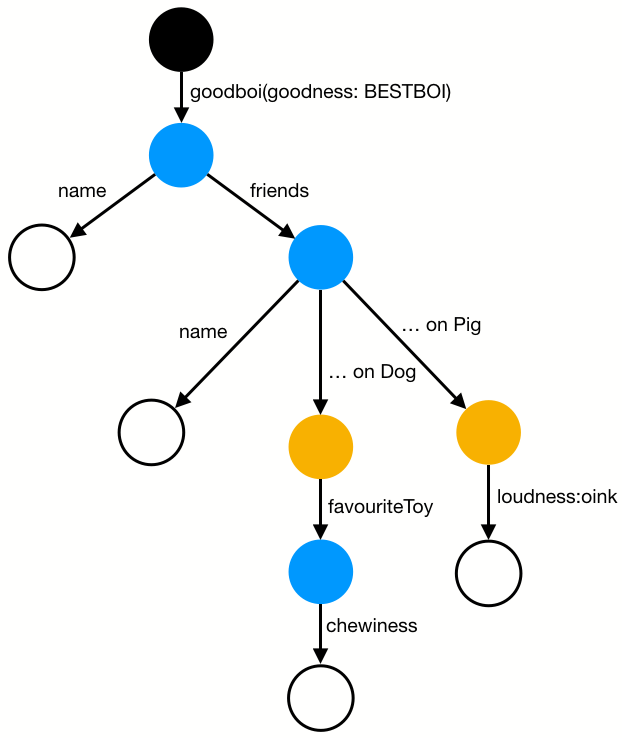
\includegraphics[scale=0.33]{imgs/query_tree.png}
    \caption{GraphQL query as a tree.}
    \label{fig:query_tree}
\end{figure}

Similar to the schema definition, we try to follow the Spec's grammar as close as possible. The grammar can be described as follows\td{It actually is a tiny bit different but unnecessarily... this captures it}:
\begin{grammar}
    <Query> ::= <name> \textbf{(} <Arg>* \textbf{)}
    \alt <alias> \textbf{:} <name> \textbf{(} <Arg>* \textbf{)}
    \alt <name> \textbf{(} <Arg>* \textbf{)} \textbf{\{} <Query>+ \textbf{\}}
    \alt <alias> \textbf{:} <name> \textbf{(} <Arg>* \textbf{)} \textbf{\{} <Query>+ \textbf{\}}
    \alt \textbf{... on} <name> \textbf{\{} <Query>+ \textbf{\}}
    
    <Arg> ::= <name> \textbf{:} <value>
\end{grammar}
    
And the implementation in GraphCoQL is the following.\td{Not sure how to display this.}

\begin{minted}{coq}
Inductive Query : Type :=
| SingleField (name : Name)
              (arguments : seq (Name * Vals))
            
| AliasedField (alias : Name)
               (name : Name)
               (arguments : seq (Name * Vals))
             
| NestedField (name : Name)
              (arguments : seq (Name * Vals))
              (subqueries : seq Query)
            
| NestedAliasedField (alias : Name)
                     (name : Name)
                     (arguments : seq (Name * Vals))
                     (subqueries : seq Query)

| InlineFragment (type_condition : Name)
                 (subqueries : seq Query).
\end{minted}

\td{PH includes a rule for list of queries at the same level as the other rules. The issue with this is that it allows building arbitrary tree instead of just a list of queries. They can be flattened but it's something they just assume I believe.}

Before evaluating queries, they must go through a validation process. This is similar to the \textit{well-formedness} of schemas or \textit{conformance} of graphs. Whenever we validate queries, there is always a notion of a type in context. This is the type to which we might be requesting information on its fields\footnote{At top level, this would be the query type.}. Requesting a field might be valid in a certain type but not in others. Similarly, a field may have a particular return type in one case and a different one in another type. Due to space constraints, we do not include the complete definitions.

\begin{definition}
A GraphQL query $\varphi$ conforms to a schema $\mathcal{S}$ if it satisfies the following conditions:
\begin{itemize}
    \item Selections in $\varphi$ are consistent by themselves. This notion includes things such as: if we query a field, then that field is defined in the  type in context and its arguments are defined in the given field, or if it is an inline fragment, then the type condition has to be valid wrt. the type in context. 
    
    \item Field merging between fields is possible. During the evaluation process, fields with the same response name are collected and merged to ensure that they are all executed at the same time. This validation rule checks that it makes sense to merge those fields. The following example illustrates two queries that have the same response name but should not be merged. The first one is accessing the field \texttt{name} while the second is accessing the field \texttt{age} but renaming it to \texttt{name}. Both are selections on different fields of the same type but with the same response name.
    \begin{minted}{gql.py:GraphqlLexer -x}
                    query {
                        name
                        name:age
                    }
    \end{minted}
    
    \item Fields with same response name have compatible response shapes. This checks whether two fields with the same response name will produce response values that are consistent to each other. These values should be unambiguous for a user. For instance, the following example\td{These examples look a bit off I think.} shows two queries that produce similar responses but with ambiguous values. In the first one, we ask for dog's \texttt{name}s, which are strings, and in the second for pig's \texttt{age}s, which are integers. We also rename the \texttt{age} value to \texttt{name}. The responses we get will have some cases where \texttt{name} is associated to a string and other where it is associated to integers.
    \begin{minted}[escapeinside=||,mathescape=true]{gql.py:GraphqlLexer -x}
                    query {
                        |$\ldots$| on Dog {
                            name
                        }
                        |$\ldots$| on Pig {
                            name:age
                        }
                    }
    \end{minted}
\end{itemize}
\end{definition}

\begin{minted}{coq}
Definition queries_conform (type_in_scope : Name) 
                           (queries : seq Query) : bool :=
        all (is_consistent type_in_scope) queries &&
        is_field_merging_possible type_in_scope queries &&
        have_compatible_response_shapes 
            [seq (type_in_scope, q) | q <- queries].
\end{minted}

Finally, with these definitions we can build queries in a GraphQL service. From now on, we will assume that queries are well-formed with respect to a given schema. We can then move onto their semantics.

\subsection{Semantics}\label{subsec:semantics}

We are now ready to review how queries are evaluated. We will begin by briefly reviewing the responses generated by executing our queries. Then we will give an informal description of our semantics, followed by the formal definition. We will finish by discussing some implementation choices and comparison with the Spec and HP.

We chose to model responses as a tree structure, similar to JSON. The Spec only states that responses must be a map. We chose this structure because it is similar to the one used by queries and because it is simpler to preserve order of the responses. The ordering of responses is not a hard requirement but it is one of the selling points for GraphQL (queries and their responses are very similar and easy to read). We use option types to represent null values in the leaves of the response tree.

\begin{minted}{coq}
Inductive ResponseNode : Type :=
| Leaf : A -> ResponseNode
| Object : seq (Name * ResponseNode) -> ResponseNode
| Array : seq ResponseNode -> ResponseNode.

Variable (Vals: eqType).

Definition GraphQLResponse := 
    seq (Name * (@ResponseNode (option Vals))).
\end{minted}

Moving onto the semantics of GraphQL queries. We chose to model it similarly to HP, in the sense that our data model is a graph. Therefore, a query represents a navigation over an underlying graph. At top level, our query starts from the root node and then moves around its edges and nodes, collecting data along its way. In this sense:
\begin{itemize}
    \item A field selection represents one of two things: accessing a node's property or traversing an edge to a neighboring node. On the neighboring nodes we recursively evaluate the subqueries.
    \item An inline fragment conditions whether we access some value of a node or if we use it to traverse to other nodes.
\end{itemize}

Figure \ref{fig:semantics} shows the formal definition of the semantics. It displays the cases where a field selection is accessing a node's property, when it is navigating to other nodes or when it is evaluating an inline fragment. Aliased fields are omitted for brevity.

\begin{figure*}
    \centering
    \begin{align} 
    % Empty
    \eval{\cdot}{u} &= [\cdot] \\
    % SingleField
    \evalu{\fld\; ::\; \queries} &= \begin{cases}
    \resp{\val} \; ::\; \evalfilteru{\queries}{\fkey}  & \mathit{u.property}(\fld) = \val \\
    \resp{\nval} \; :: \; \evalfilteru{\queries}{\fkey} & \sim
    \end{cases}\\
    % Nested field
    \evalu{\nfld{\overline{\beta}} \; ::\; \queries} &=
    \begin{cases}
    \resp{\texttt{[} \mathit{map} (\lambda\; v_{i} \Rightarrow \eval{\overline{\beta} \mdoubleplus \mathit{merge (collect_\fkey (\queries))}}{v_{i}})\; \mathit{neighbors(u)} \texttt{]}} \; :: \; \evalfilteru{\queries}{f}  & \mathit{type(f)} \in L_{t} \text{and} \{v_{1}, \ldots, v_{k}\} = \{v_{i} \mid (u, f[\alpha], v_{i}) \in E\} \\
    (f:\{\eval{\subqueries{\beta}}{v}\})\; :: \; \evalfilteru{\queries}{f}  & \mathit{type(f)} \notin L_{t} \text{and} (u, f[\alpha], v) \in E \\
    (f:null)\; :: \; \evalfilteru{\queries}{f} & \mathit{type(f)} \notin L_{t} \text{and there is no } v \text{ s.t.} (u, f[\alpha], v) \in E \\
    \end{cases}\\
    %inline fragment
    \evalu{\ifrag{t}{\overline{\beta}}\; ::\; \queries} &= \begin{cases}
    \evalu{\overline{\beta} \mdoubleplus \queries} & \mathit{does\_fragment\_type\_apply_{\texttt{t}}(u.type)} = \texttt{true}\\
    \evalu{\queries} & \sim
    \end{cases}
    \end{align}
    \caption{Semantics for GraphQL queries.\td{This looks bad but I don't know how to format it :/}}
    \label{fig:semantics}
\end{figure*}
There are two major aspects that we need to address about our formalization; errors and completeness.

The first one is that we currently do not handle errors during execution. This is due to two main reasons: our semantics assumes it receives valid queries and we have not yet implemented non-null types. These relates to the two kinds of errors one may encounter: validation and execution errors. The first ones are captured before execution and displayed to the user. Our semantics has to deal with a case which would be ruled out by the validation process. We believe both cases can be covered by including X (monad/reasonably exceptional type theory/etc)\td{rewrite}.

The second major aspect refers to completeness. Our semantics does not cover all possible responses expected by a GraphQL service. In particular, it does not account for list types of depth bigger than one, when its inner type is not a scalar type\footnote{HP goes a step further and does not allow any type of nested list result.}. For instance, one might want to get information about friends but grouped by their age. This could be modeled as a field with type \texttt{[[Human]]}, where the list type has depth 2. A response for this query would look something like \texttt{"friends":[[...], ..., [...]]}. This response cannot be generated by our semantics\footnote{It can be defined with the \mintinline{coq}{Response} structure but not generated with the semantics.}.

The main challenge in this case is to define what this nested list types represent in a graph. If we take a simple case of a field with type \texttt{[Human]}, we can model it as neighbors of a node. However, if we increase the nesting such as \texttt{[[Human]]}, it becomes harder to model. What does this represent in the graph? Should we introduce blank nodes in between the source node and the \texttt{Human} nodes? Are these inner edges labeled? Should there be a blank node per each level of nesting or a single one with edges to itself? All these questions do not have a straightforward answer. Our semantics, as the one definded in PH, simply ignores any nesting bigger than one.\td{This is where it can be modelled using Functors. The Spec checks if it received a collection and applies map to eventually get to the concrete values. Not sure how to put this out there.}

This concludes the base formalization of GraphQL schemas, graph data model, and queries and their semantics. Using this basic structures we can start defining query transformations and prove some properties about them. 
